\documentclass[12pt]{article}
\usepackage[table]{xcolor}
\usepackage[shortlabels]{enumitem}
\usepackage{tabularx,xltabular}
\usepackage{graphicx}
\usepackage{hyperref}
\usepackage{verbatim}
\usepackage{geometry}
\usepackage{ulem}
\usepackage[official]{eurosym}
\usepackage{tikz}
\usetikzlibrary{arrows,backgrounds,calc,decorations.markings,patterns,3d}
\usepackage{pgfplots}
\pgfplotsset{compat = newest}
\usetikzlibrary{fit}
\newcommand\addvmargin[1]{
\usetikzlibrary{arrows}
\node[fit=(current bounding box),inner ysep=#1,inner xsep=0]{};}
\usepackage{cancel}
\usepackage{fontspec}
\usepackage{array}  
\geometry{a4paper, top=2cm, left=2cm, right=2cm, bottom=2cm, headsep=1cm}
\usepackage{tabu}
\usepackage{pst-node}
\usepackage{colortbl}
\usepackage{array}
\usepackage{german}
\setlength\parindent{0pt}
\newcolumntype{?}{!{\vrule width 1pt}}
\usepackage{makecell}
\renewcommand{\arraystretch}{2.5}
\usepackage{pbox}
\usepackage{amssymb}
\usepackage{amsmath}
\usepackage{booktabs}
\newcolumntype{L}[1]{>{\raggedright\let\newline\\\arraybackslash\hspace{0pt}}m{#1}}
\newcolumntype{C}[1]{>{\centering\let\newline\\\arraybackslash\hspace{0pt}}m{#1}}
\newcolumntype{R}[1]{>{\raggedleft\let\newline\\\arraybackslash\hspace{0pt}}m{#1}}
\begin{document}
\rightline{Datum: 07.06.2023}
\centerline{{\Large Einfache Gleichung lösen}} 
\vspace{1cm}
\noindent \\


\begin{xltabular}{\textwidth}{|C{0.75cm}|X|C{0.75cm}|X|}
\arrayrulecolor{black}\hline
a)&Berechne die Variable$$b+11 = 21$$
&
b)&Berechne die Variable$$x+50 = 5$$
\\\hline
c)&Berechne die Variable$$y+49 = 43$$
&
d)&Berechne die Variable$$y-46 = 48$$
\\\hline
\end{xltabular}
\vspace{0.5cm}
\newpage
\rightline{Datum: 07.06.2023}
\centerline{{\large Lösungen Einfache Gleichung lösen}} 
\vspace{0.5cm}

\begin{xltabular}{\textwidth}{|C{0.75cm}|X|C{0.75cm}|X|}
\arrayrulecolor{black}\hline
a)&\begingroup\setlength{\jot}{-0.03cm}
\tikzstyle{background grid}=[draw, black!15,step=.5cm]
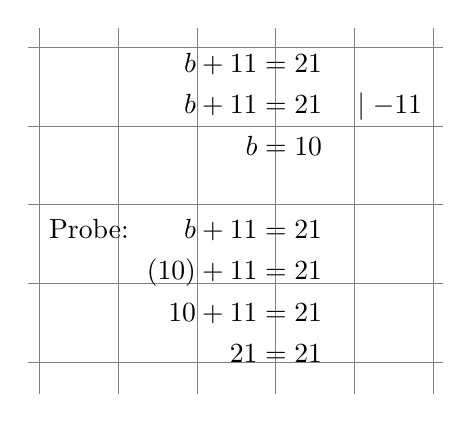
\begin{tikzpicture}[show background grid]
\node[below right] at (0,0.1) {
$\begin{aligned}
b+11  &= 21& &  \\
b + 11 &=21& & \mid - 11\\
b &=10& & 
\\
\\
\mbox{Probe:}\qquad b+11  &= 21& &  \\
\left(10\right)+11  &= 21& &  \\
10+11 &=21& &  \\
21 &=21& &  \\
\end{aligned}$};
\end{tikzpicture}
\endgroup
&
b)&\begingroup\setlength{\jot}{-0.03cm}
\tikzstyle{background grid}=[draw, black!15,step=.5cm]
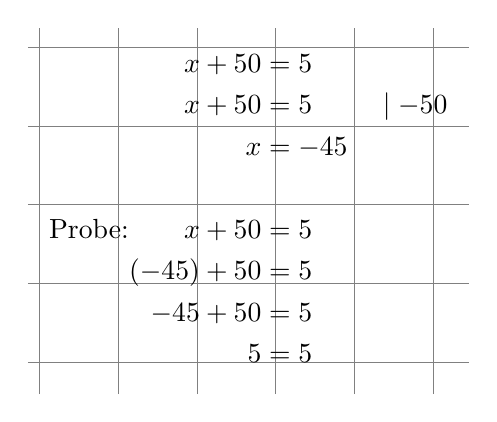
\begin{tikzpicture}[show background grid]
\node[below right] at (0,0.1) {
$\begin{aligned}
x+50  &= 5& &  \\
x + 50 &=5& & \mid - 50\\
x &=-45& & 
\\
\\
\mbox{Probe:}\qquad x+50  &= 5& &  \\
\left(-45\right)+50  &= 5& &  \\
-45+50 &=5& &  \\
5 &=5& &  \\
\end{aligned}$};
\end{tikzpicture}
\endgroup
\\\hline
c)&\begingroup\setlength{\jot}{-0.03cm}
\tikzstyle{background grid}=[draw, black!15,step=.5cm]
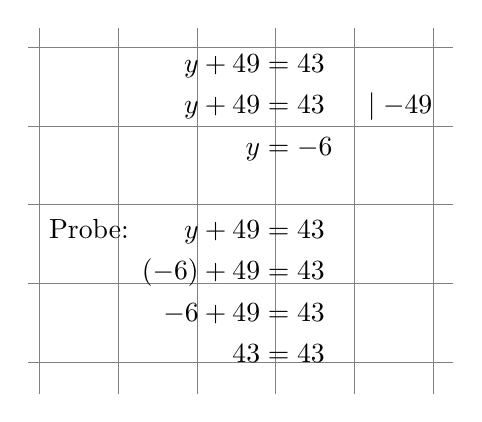
\begin{tikzpicture}[show background grid]
\node[below right] at (0,0.1) {
$\begin{aligned}
y+49  &= 43& &  \\
y + 49 &=43& & \mid - 49\\
y &=-6& & 
\\
\\
\mbox{Probe:}\qquad y+49  &= 43& &  \\
\left(-6\right)+49  &= 43& &  \\
-6+49 &=43& &  \\
43 &=43& &  \\
\end{aligned}$};
\end{tikzpicture}
\endgroup
&
d)&\begingroup\setlength{\jot}{-0.03cm}
\tikzstyle{background grid}=[draw, black!15,step=.5cm]
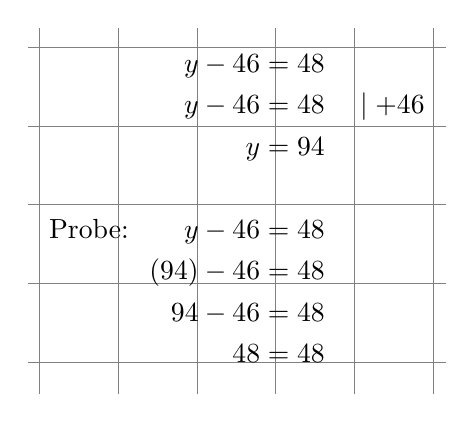
\begin{tikzpicture}[show background grid]
\node[below right] at (0,0.1) {
$\begin{aligned}
y-46  &= 48& &  \\
y - 46 &=48& & \mid + 46\\
y &=94& & 
\\
\\
\mbox{Probe:}\qquad y-46  &= 48& &  \\
\left(94\right)-46  &= 48& &  \\
94-46 &=48& &  \\
48 &=48& &  \\
\end{aligned}$};
\end{tikzpicture}
\endgroup
\\\hline
\end{xltabular}
\vspace{0.5cm}
\end{document}